%! TEX root = supplementary.tex
\newcommand{\iw}{1cm}
\newcommand{\cw}{\textwidth}
\begin{figure*}[h]
	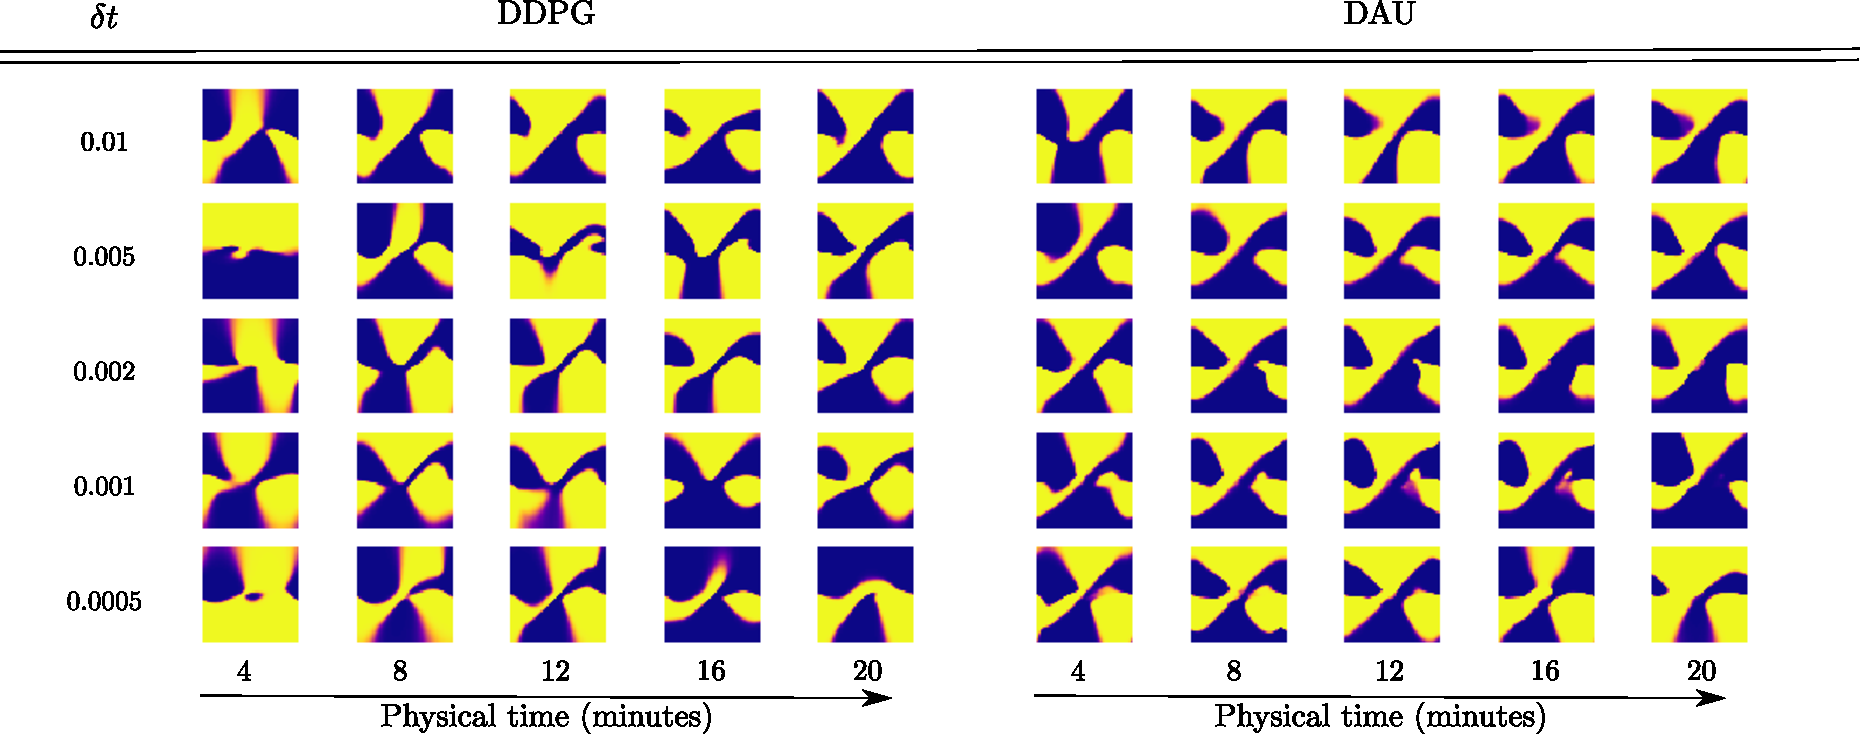
\includegraphics[width=\cw]{figs_data/pendulum_unscaled/pendulum_fig_act_unscaled.pdf}
	\caption{Policies obtained by DDPG (unscaled version) and AU at different instants in physical time of training on the pendulum swing-up environment. Each image represents the policy learnt by the policy network, with $x$-axis representing angle, and $y$-axis angular velocity. The lighter the pixel, the closer to $1$ the action, the darker, the closer to $-1$.}
        \label{fig:pend}
\end{figure*}
\begin{figure*}[h]
	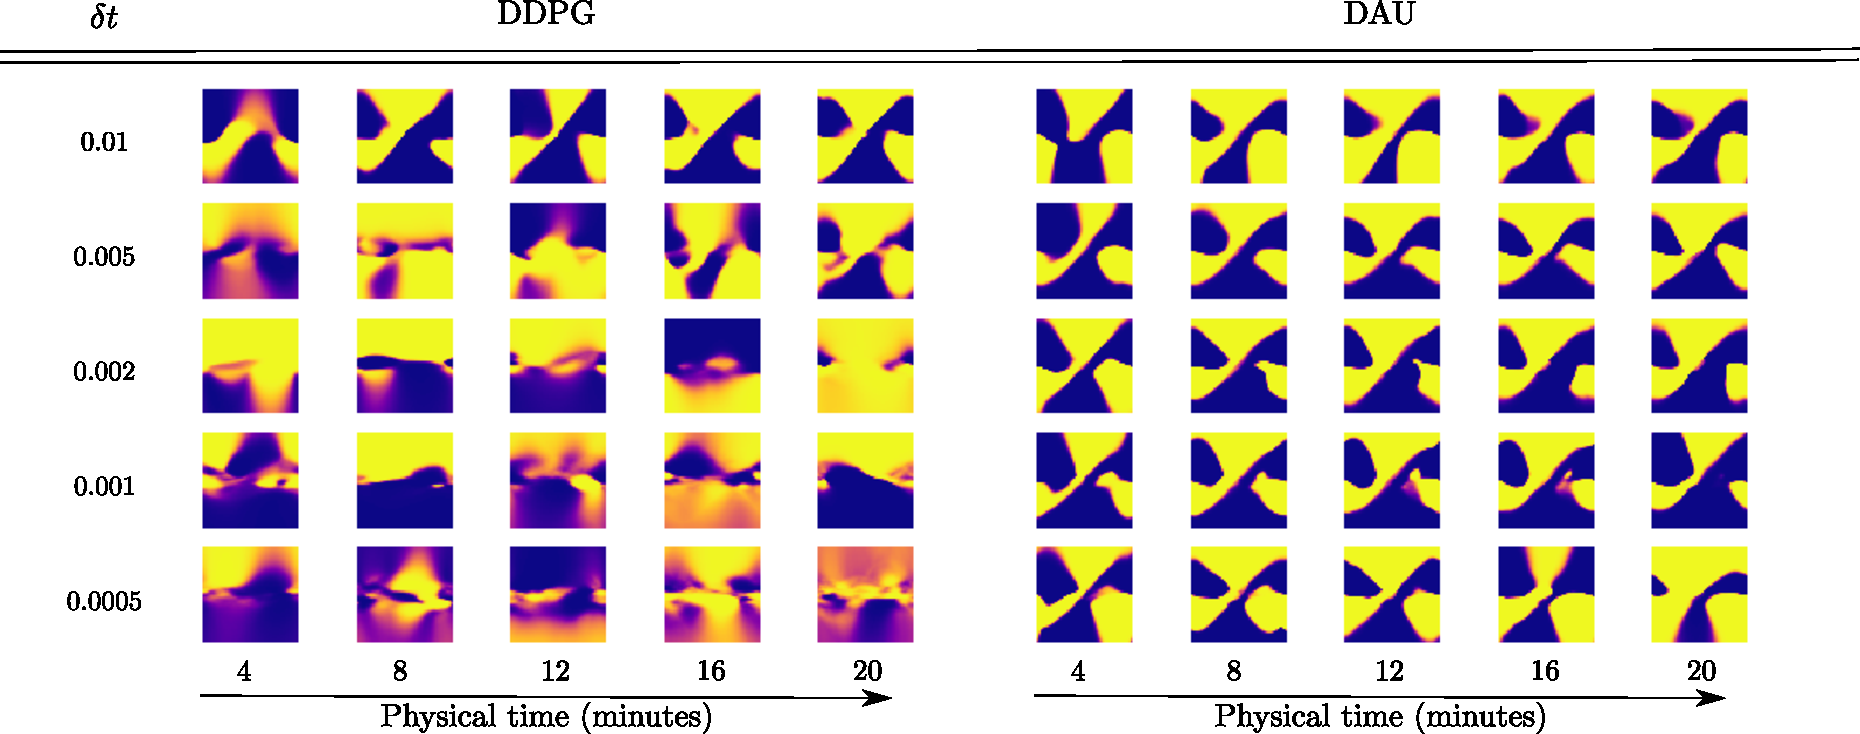
\includegraphics[width=\cw]{figs_data/pendulum_scaled/pendulum_fig_act_scaled.pdf}
	\caption{Policies obtained by DDPG (scaled version) and AU at different instants in physical time of training on the pendulum swing-up environment. Each image represents the policy learnt by the policy network, with $x$-axis representing angle, and $y$-axis angular velocity. The lighter the pixel, the closer to $1$ the action, the darker, the closer to $-1$.}
        \label{fig:pend}
\end{figure*}
\begin{figure*}[h]
	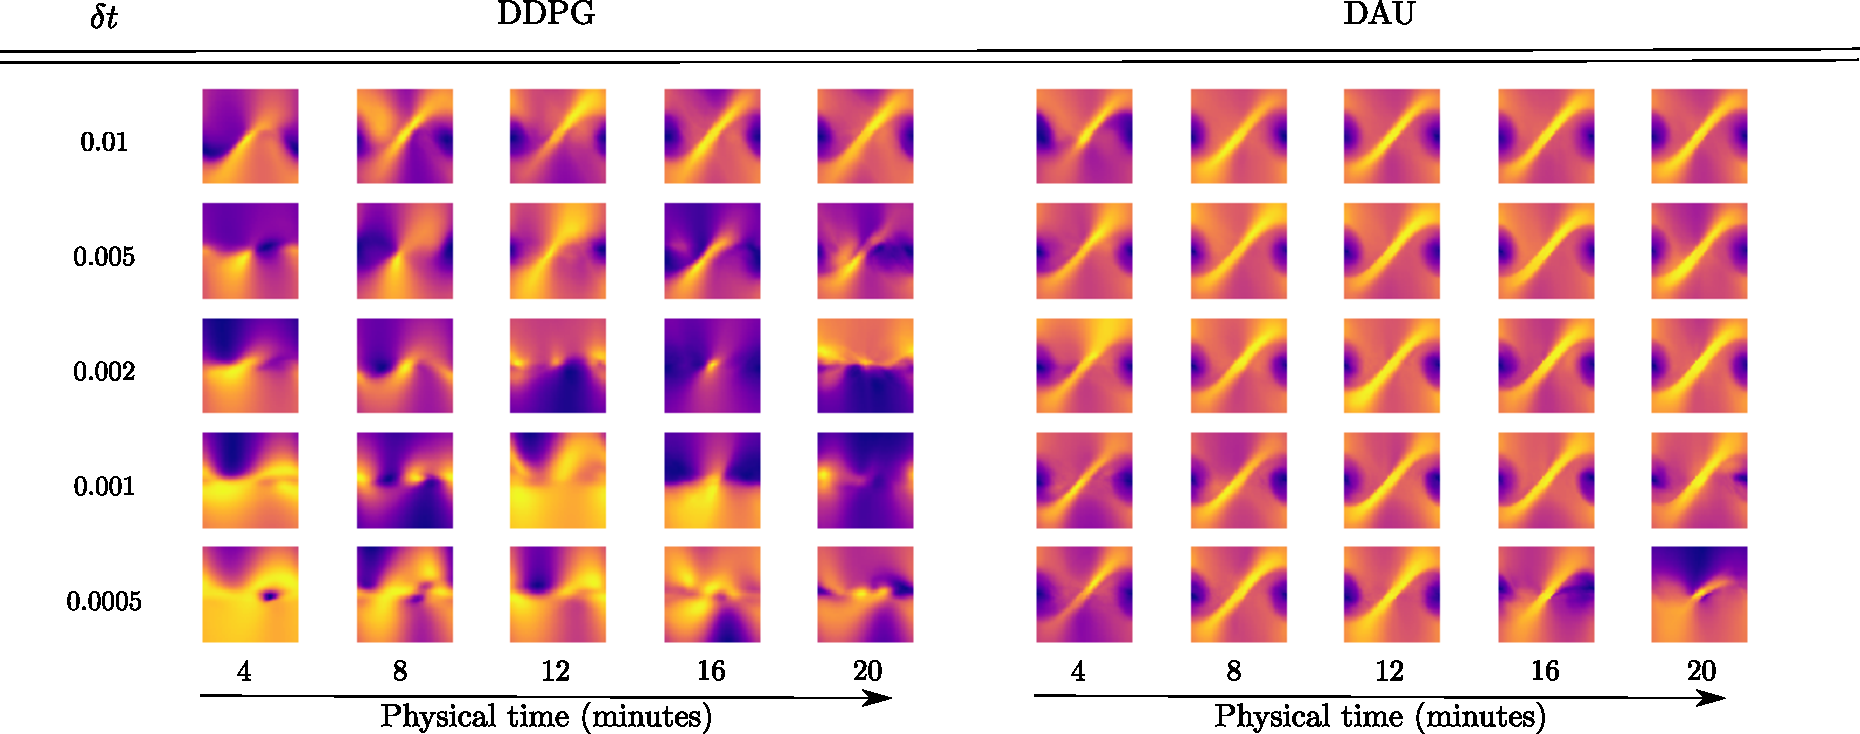
\includegraphics[width=\cw]{figs_data/pendulum_scaled/pendulum_fig_val_scaled.pdf}
	\caption{Value functions obtained by DDPG (scaled version) and AU at different instants in physical time of training on the pendulum swing-up environment. Each image represents the policy learnt by the policy network, with $x$-axis representing angle, and $y$-axis angular velocity. The lighter the pixel, the closer to $1$ the action, the darker, the closer to $-1$.}
        \label{fig:pend}
\end{figure*}
